\documentclass[border=4pt,tikz]{standalone}
\usepackage[T1]{fontenc}
\usepackage{lmodern}
\usetikzlibrary{positioning,arrows.meta,calc,fit,backgrounds,patterns}
% Shared visual language for the paper's architecture diagrams.
% Every fill differs in lightness, so the diagrams stay legible when printed
% in grayscale; colour is only a redundant cue.
\definecolor{ink}{HTML}{1B2A3A}
\definecolor{navyfill}{HTML}{D5E0EC}
\definecolor{navyedge}{HTML}{2F5D8A}
\definecolor{tealfill}{HTML}{BFD8D5}
\definecolor{tealedge}{HTML}{2A6F6C}
\definecolor{amberfill}{HTML}{F1DCAE}
\definecolor{amberedge}{HTML}{9C6512}
\definecolor{greyfill}{HTML}{E5E7EB}
\definecolor{greymid}{HTML}{8B939E}
\definecolor{redfill}{HTML}{F0CBC5}
\definecolor{rededge}{HTML}{9E3B32}

\tikzset{
  >={Stealth[length=2.0mm,width=1.5mm]},
  every node/.style={font=\footnotesize, text=ink},
  box/.style={draw=ink, line width=0.5pt, rounded corners=1.5pt,
              fill=greyfill, align=center, inner sep=3pt, minimum height=7mm},
  databox/.style={box, fill=amberfill, draw=amberedge},
  procbox/.style={box, fill=navyfill, draw=navyedge},
  repbox/.style={box, fill=tealfill, draw=tealedge},
  evalbox/.style={box, fill=redfill, draw=rededge},
  fadebox/.style={box, fill=white, draw=greymid, dashed},
  arr/.style={->, draw=ink, line width=0.6pt},
  darr/.style={->, draw=greymid, line width=0.6pt, dashed},
  lbl/.style={font=\scriptsize, text=ink, inner sep=1pt, fill=white, fill opacity=0.85, text opacity=1},
  note/.style={font=\scriptsize, text=ink, align=left, inner sep=1pt},
  badge/.style={draw=rededge, fill=redfill, rounded corners=6pt,
                font=\scriptsize\bfseries, text=rededge, inner sep=2.2pt},
  badgefrz/.style={draw=tealedge, fill=tealfill, rounded corners=6pt,
                font=\scriptsize\bfseries, text=tealedge, inner sep=2.2pt},
  group/.style={draw=greymid, line width=0.5pt, rounded corners=3pt, inner sep=6pt},
}


% NOTE: TikZ node text must not wrap a multi-line block in braces: `\\` inside
% a brace group is not the node line-break. Keep node text flat. Every node has
% an explicit text width so that box widths are deterministic and the layout
% does not self-collide.
\begin{document}
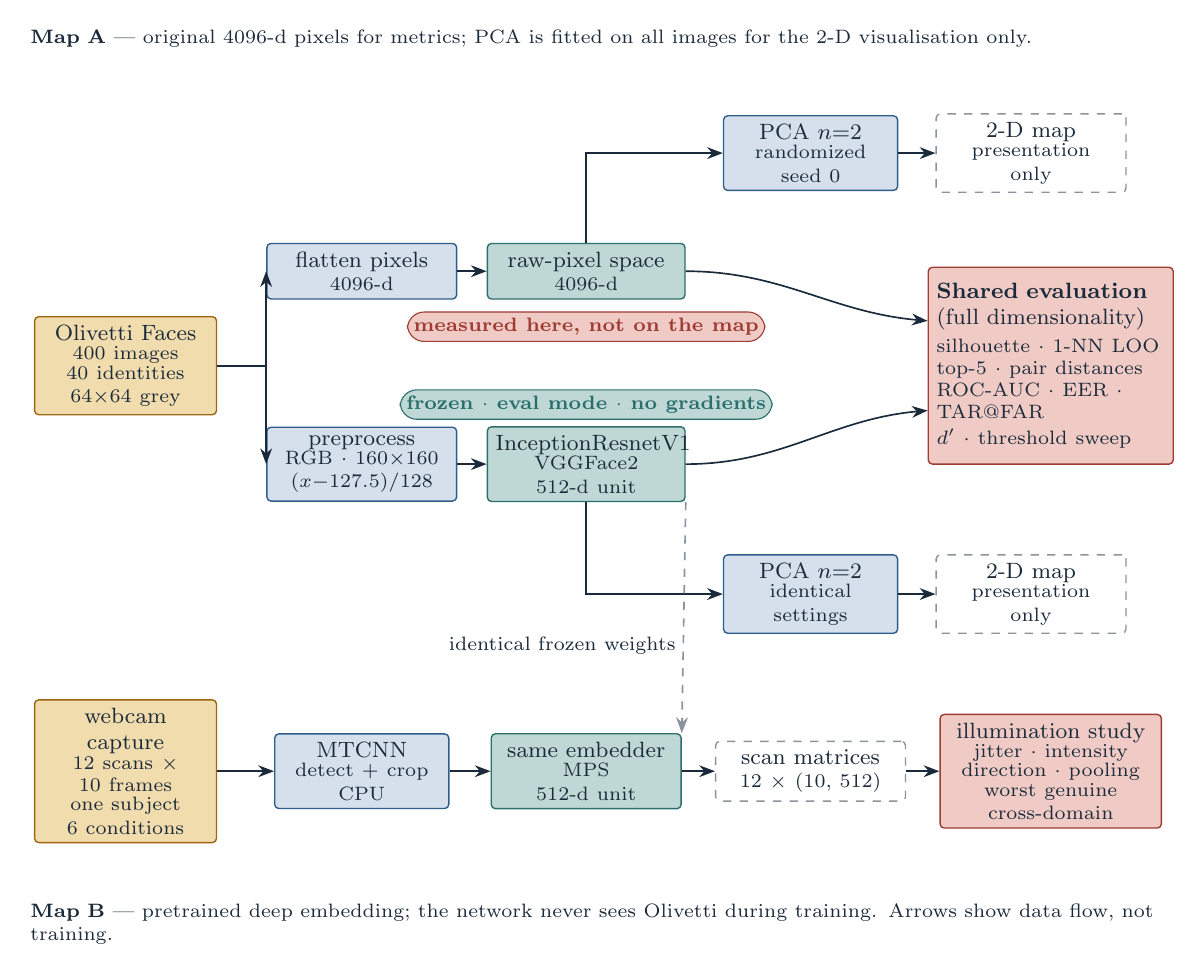
\begin{tikzpicture}[x=1cm,y=1cm]

% ---------------------------------------------------------------- data source
\node[databox, text width=2.1cm] (oliv) at (1.25,1.25)
  {Olivetti Faces\\[-1pt] \scriptsize 400 images\\[-1pt] \scriptsize 40 identities\\[-1pt] \scriptsize 64$\times$64 grey};

% ---------------------------------------------------------------- Map A lane
\node[procbox, text width=2.2cm] (flat) at (4.25,2.45)
  {flatten pixels\\[-1pt] \scriptsize 4096-d};
\node[repbox, text width=2.3cm] (raw) at (7.10,2.45)
  {raw-pixel space\\[-1pt] \scriptsize 4096-d};
\node[procbox, text width=2.0cm] (pcaA) at (9.95,3.95)
  {PCA $n{=}2$\\[-1pt] \scriptsize randomized\\[-1pt] \scriptsize seed 0};
\node[fadebox, text width=2.2cm] (mapA) at (12.75,3.95)
  {2-D map\\[-1pt] \scriptsize presentation\\[-1pt] \scriptsize only};

% ---------------------------------------------------------------- Map B lane
\node[procbox, text width=2.2cm] (prep) at (4.25,0.00)
  {preprocess\\[-1pt] \scriptsize RGB $\cdot$ 160$\times$160\\[-1pt] \scriptsize $(x{-}127.5)/128$};
\node[repbox, text width=2.3cm] (emb) at (7.10,0.00)
  {InceptionResnetV1\\[-1pt] \scriptsize VGGFace2\\[-1pt] \scriptsize 512-d unit};
\node[procbox, text width=2.0cm] (pcaB) at (9.95,-1.65)
  {PCA $n{=}2$\\[-1pt] \scriptsize identical\\[-1pt] \scriptsize settings};
\node[fadebox, text width=2.2cm] (mapB) at (12.75,-1.65)
  {2-D map\\[-1pt] \scriptsize presentation\\[-1pt] \scriptsize only};

% ---------------------------------------------------------------- live lane
\node[databox, text width=2.1cm] (cam) at (1.25,-3.90)
  {webcam capture\\[-1pt] \scriptsize 12 scans $\times$ 10 frames\\[-1pt] \scriptsize one subject\\[-1pt] \scriptsize 6 conditions};
\node[procbox, text width=2.0cm] (mtcnn) at (4.25,-3.90)
  {MTCNN\\[-1pt] \scriptsize detect + crop\\[-1pt] \scriptsize CPU};
\node[repbox, text width=2.2cm] (emb2) at (7.10,-3.90)
  {same embedder\\[-1pt] \scriptsize MPS\\[-1pt] \scriptsize 512-d unit};
\node[fadebox, text width=2.2cm] (scans) at (9.95,-3.90)
  {scan matrices\\[-1pt] \scriptsize 12 $\times$ (10, 512)};
\node[evalbox, text width=2.6cm] (live) at (13.00,-3.90)
  {illumination study\\[-1pt] \scriptsize jitter $\cdot$ intensity\\[-1pt] \scriptsize direction $\cdot$ pooling\\[-1pt] \scriptsize worst genuine\\[-1pt] \scriptsize cross-domain};

% ---------------------------------------------------------------- evaluation
\node[evalbox, text width=2.9cm, minimum height=25mm, align=left] (eval) at (13.00,1.25)
  {\textbf{Shared evaluation}\\ (full dimensionality)\\[2pt] \scriptsize silhouette $\cdot$ 1-NN LOO\\ \scriptsize top-5 $\cdot$ pair distances\\ \scriptsize ROC-AUC $\cdot$ EER $\cdot$ TAR@FAR\\ \scriptsize $d'$ $\cdot$ threshold sweep};

% ---------------------------------------------------------------- arrows
\draw[arr] (oliv.east) -| (flat.west);
\draw[arr] (oliv.east) -| (prep.west);
\draw[arr] (flat) -- (raw);
\draw[arr] (prep) -- (emb);
\draw[arr] (raw.north) |- (pcaA.west);
\draw[arr] (pcaA) -- (mapA);
\draw[arr] (emb.south) |- (pcaB.west);
\draw[arr] (pcaB) -- (mapB);
\draw[arr] (raw.east) to[out=0,in=175] (eval.160);
\draw[arr] (emb.east) to[out=0,in=185] (eval.200);

\draw[arr] (cam) -- (mtcnn);
\draw[arr] (mtcnn) -- (emb2);
\draw[arr] (emb2) -- (scans);
\draw[arr] (scans) -- (live);
\draw[darr] (emb.south east) -- node[lbl, left=1.5pt, pos=0.62] {identical frozen weights} (emb2.north east);

% ---------------------------------------------------------------- badges / notes
\node[badgefrz, above=0.8mm of emb] {frozen $\cdot$ eval mode $\cdot$ no gradients};
\node[badge, below=1.5mm of raw] {measured here, not on the map};
\node[note, anchor=north west, text width=14.5cm] at (0.0,5.55)
  {\textbf{Map A} --- original 4096-d pixels for metrics; PCA is fitted on all images for the 2-D visualisation only.};
\node[note, anchor=north west, text width=14.5cm] at (0.0,-5.55)
  {\textbf{Map B} --- pretrained deep embedding; the network never sees Olivetti during training. Arrows show data flow, not training.};

\end{tikzpicture}
\end{document}
